\documentclass[14pt]{article}
\usepackage{graphicx}

\usepackage{multirow}
\usepackage{verse}
\newcommand{\attrib}[1]{%
\nopagebreak{\raggedright\footnotesize #1\par}}
\renewcommand{\poemtitlefont}{\normalfont\large\itshape\centering}
 
\usepackage{chemfig}
\usepackage{circuitikz}
\usepackage{amsmath}

\usepackage{pgfplots}
\pgfplotsset{width=7cm,compat=1.8}

\usepackage{geometry}

\usepackage[%
  newcommands     % \RaggedRight=\raggedright etc. 
 ,newparameters   % use default settings of ragged2e
]{ragged2e}
\usepackage[pdfauthor={Sina Ahmadi},
            pdftitle={Using XeLaTeX for Kurdish}]{hyperref}
            
\hypersetup{colorlinks,breaklinks,
            urlcolor=[rgb]{0,0.5,0.5},
            linkcolor=[rgb]{0,0.5,0.5}}

\usepackage{listings}
\lstset{%
language={[LaTeX]TeX},
numbersep=5mm,
basicstyle=\footnotesize,
numbers=left,
stepnumber=1,
numberstyle=\tiny,
breaklines=true,frame=single,framexleftmargin=2mm, xleftmargin=2mm,
prebreak = \raisebox{0ex}[0ex][0ex]{\ensuremath{\hookleftarrow}},
backgroundcolor=\color{green!5},frameround=fttt,escapeinside=??,
rulecolor=\color{red},
morekeywords={
    maketitle},
keywordstyle=\color[rgb]{0,0,1},                    
        commentstyle=\color[rgb]{0.133,0.545,0.133},
        stringstyle=\color[rgb]{0.627,0.126,0.941}
%columns=fullflexible
}


% numerals: eastern and western

\usepackage{polyglossia}
\setdefaultlanguage[variant=sorani,script=Arabic,numerals=eastern]{kurdish}
\newfontfamily\arabicfont[Script=Arabic,Scale=1]{Yas}
%\newfontfamily\arabicfont[Script=Arabic]{Amiri}%
\let\arabicfonttt\ttfamily
\setotherlanguage{english}
\setotherlanguage[variant=poly]{greek}
\newfontfamily\greekfont{Times New Roman}[Script=Greek]
\newfontfamily\kurdishfont[Script=Arabic,Scale=1,Ligatures=Contextual]{Yas}


\title{ \XeLaTeX~بۆ نووسینی کوردی}
\author{سینا ئەحمەدی \\ {\small \texttt{ahmadi.sina@outlook.com} } \\ {\small \url{https://sinaahmadi.github.io/}}}
\date{\today}

\begin{document}

\maketitle
\tableofcontents

\begin{abstract}

ماوەیەک بوو خولیای ئەوەم هەبوو کە بتوانم 
\textenglish{\TeX} بۆ نووسینی کوردی بە کار بێنم. هەر ئەوە هانی دام کە خۆم کوردی لێ زیاد بکەم.
لەم بەڵگەیەدا باس لە بەکار هێنانی \textenglish{\XeLaTeX} لەگەڵ پەکەیجی 
\texttt{\textenglish{Polyglossia}}
 بۆ نووسینی کوردی دەکەم.
 لە دوایین وەشانی کوردی لەم پەکەیجەدا، دوو زاراوەی سۆرانی و کرمانجی بە هەر دوو ڕێنووسی لاتین و عەرەبی دابین کراون.
دڵنیام ئەگەر بە باشی فێری \textenglish{\TeX} بن، دەزانن چێژێک کە لە بەکارهێنانی \textenglish{\TeX}دا هەیە لە چ بەرنامەی دیکەدا نییە!
\end{abstract}

\section{\textenglish{\TeX} چییە؟}

\textenglish{\TeX} سیستەمێکی ئامادەکردنی بەڵگەیە کە تێیدا نووسەر لە دەقی ساکار لەگەڵ نیشانەگەلی تایبەتی بۆ نووسین کەڵک وەردەگرێ. ئەم بۆچوونە جیاوازە لە شێوازی دیکەی دەست وەردانی دەق کە تێیدا هەر شتێک بێتە چاو هەر ئەو شتەیە کە چاپ دەبێ و وەکوو ئاکامی بەڵگەکە نیشان دەدرێ. بۆیەش بە ئینگلیسی بەم شێوازە دەڵێن \textenglish{\textit{what you see is what you get}}، یان بە کورتی \textenglish{WYSIWYG}. \textenglish{Microsoft Word} نموونەیەکی ناسراوە کە لەم شێوازە کەڵک وەردەگرێ.

\textenglish{\TeX}
بۆ یەکەم جار لە ساڵی ١٩٧٨ لە لایەنی زانا و بلیمەتی کۆمپیوتەر دۆناڵد کنووس
(\textenglish{Donald Knuth})
ەوە ساز کرا.
\textenglish{\TeX} لە سەر ئەو بۆچوونەدا پێکهاتووە کە نووسەر دەبێ کاری نووسین بکا نەک ڕازاندنەوەی دەق. واتە، بۆ نووسەری بەڵگەیەک دەبێ ئەو ئامێرانە دابین کرابێ کە بتوانێ بە هەموو پێداویستییەکانی لە نووسیندا بگا، بگرە بۆ نووسینی فرمووڵێکی بیرکاری بێ یان هاوکێشەیەکی کیمیایی یان پارچە شیعرێک. بۆیەش، لە نێو ئاکادیمیا و ئەو کەسانه کە بە لێهاتوویی لە سەر بابەتێکی زانستی دەنووسن لە \textenglish{\TeX} زۆر بە بەربڵاوی کەڵک وەردەگیردرێ. 
وشەی 
\textenglish{\TeX}
 لە وشەی یۆنانی
\textgreek{\textit{τέχνη}}
یەوە
 دێ کە بە مانای هونەرە. لە بەر ئەوەی فۆنیمی 
\textgreek{χ} 
 لە کوردی و زۆر زماندا بەرانبەرێکی نییە، دەتوانین لە کوردی بڵەین
\textit{تێک} یان \textit{تێخ}.

\paragraph{تایبەتمەندییەکانی \TeX}
 بە کورتی، لە تایبەتیمەندییە هەرە گرینگەکانی تێک ئەمانەن:
 
\begin{itemize}
\item نووسینی گۆڤار، کتێب، ڕاپۆرتی تەکنیکی و سڵایدی ئامادەکاری
\item بەڕێوە بردنی بەڵگە گەورەکان کە زۆر بەش و بەند و سەرچاوەیان تێدایە
\item نووسینەوەی فرمووڵە پڕ وردەکارییەکان لە بیرکاریدا
\item سازکردنی ئۆتۆماتیکی سەرچاوەکان
\item بە ئاسانی کەڵک وەرگرتن لە وێنە و دیاگرام
\item گۆڕانەوە بە شێوەکانی دیکەی نیشان دانی دەق وەکوو HTML
\end{itemize}

هەر لە سەر بنەمای
\textenglish{\TeX}
ەوە، دواتر چەندین بەرهەمی دیکە دابین کران کە تێیاندا تایبەتمەندیگەلی زۆرتر ڕە چاو دەگیردرێ، وەکوو نووسین بە زمانانی دیکە و بە ڕێنووسی جیاواز لە ڕێنووسی لاتین. 
\textenglish{\LaTeX} 
و 
\textenglish{\XeLaTeX}
دوو نموونەی بەنێوبانگن کە بە تایبەت لەم سەردەمەدا کەڵکیان لێ وەردەگیردرێ.

\section{چۆن \TeX~بە کار بێنم؟}

بۆ کەڵک وەرگرتن لە \TeX لە سەر کۆمپیوتەرەکەت لە پێش هەموو شتێک دەبێ بەرنامەکەت دامەزراندبێ. بەڵگەیەکی ساکار بە 
\textenglish{\LaTeX} 
 لە وێنەی
\ref{fig_mwe}
دا نیشان دراوە.


\begin{figure}[h]
    \centering
    \begin{minipage}{0.29\textwidth}
        \fbox{
               \centering
        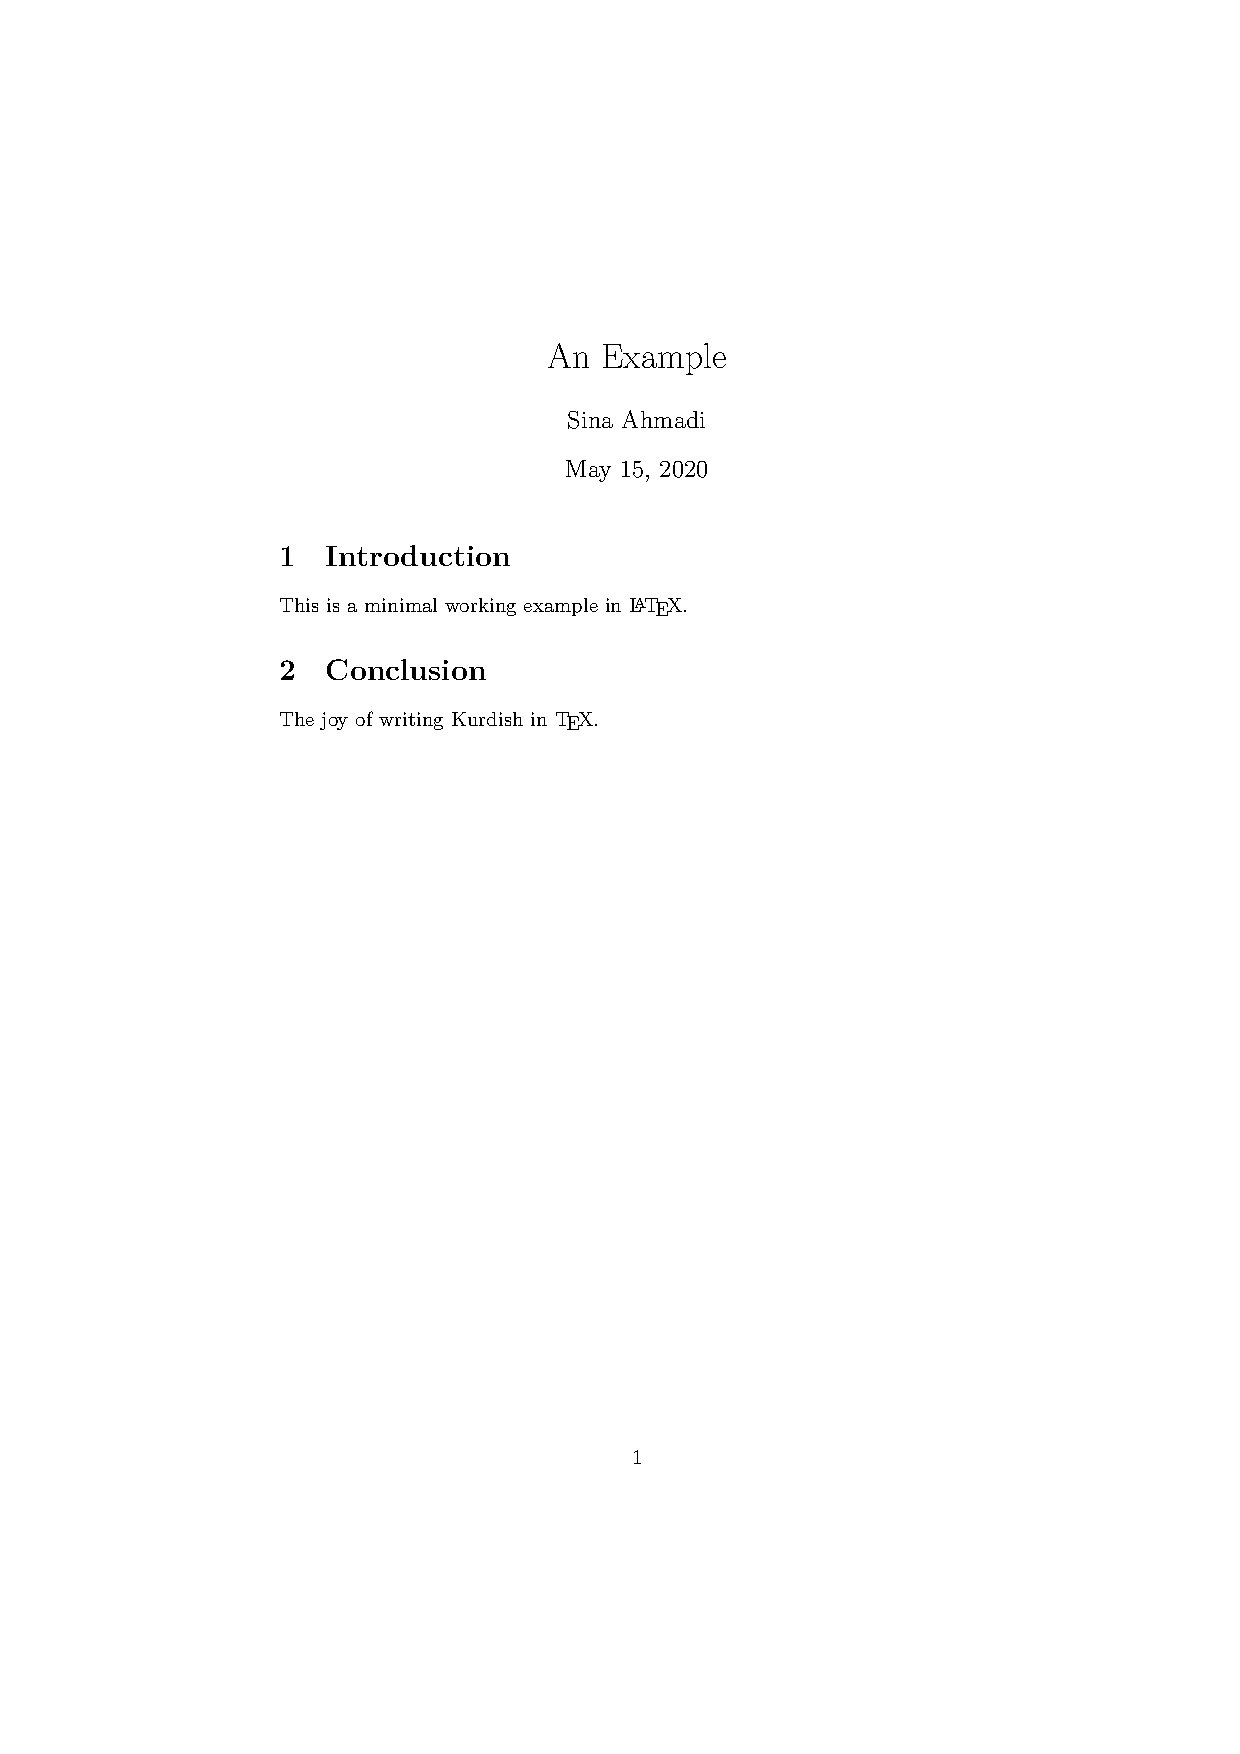
\includegraphics[width=\textwidth]{figure_example.pdf} 
        }
    \end{minipage}\hfill
    \begin{minipage}{0.65\textwidth}
\begin{english}
\begin{lstlisting}
\documentclass{article}
\usepackage[utf8]{inputenc}

\title{An Example}
\author{Sina Ahmadi}
\date{\today}

\begin{document}

\maketitle
\section{Introduction}

This is a minimal working example in \LaTeX.

\section{Conclusion}

The joy of writing Kurdish in \TeX.

\end{document}

\end{lstlisting}
\end{english}
    \end{minipage}
 \caption{نموونەیەک لە بەڵگەیەک کە بە \LaTeX~ نووسراوە. لە لای چەپەوە، کۆدی بەڵگەکەیە و لە لای ڕاستیشەوە ئاکامی کامپایل کردنیەتی}
 \label{fig_mwe}
\end{figure}



ئێستە پرسیار ئەوەیە ئایا هەر ئەم شێوەیەش دەتوانین بۆ نووسینی کوردی بە کار بێنین؟ سەرنج دەن کە لەو نموونەیەدا لە وێنەی
\ref{fig_mwe} 
کە لە سەرێ دیتمان، نە مێژوو، نە ژمارەی بەشەکان و نە تەنانەت ئەوەی کە بابەتەکە لە کوێی بەڵگەکەدا بێ و قەبارەی لاپەڕەکە چۆن بێ بە ئێمە جێبەجێ نەکراوە. واتە، \TeX بۆ خۆی بەڵگەکەمان بە هەموو ئەو وردەکارییانەوە ساز دەکا. جا بۆیە، ئەو کەسانەی کە چێژی کار کردن بە تێک دەچێژن، قەت ناتوانن بگەڕێنەوە سەر سیستمانی پێکهێنانی دەق (\textenglish{typesetting})  ی دیکە وەکوو 
\textenglish{Microsoft Office}
!
 بۆ ئەوەی زۆرتر لەگەڵ پێکهاتەکانی بەڵگەکان لە \TeX ئاشنا بن چاو لە
  \cite{wilkins1995getting} 
بکەن.


\section{\XeLaTeX~بۆ نووسینی کوردی}

 کێشەیەک کە پێشتر لە بە کار هێنانی  \TeX دا هەبوو، بە کار هێنانی زمانان و رێنووسانی دیکە بوو. \textenglish{\XeLaTeX} سیستمێکە کە لە سەر \textenglish{\TeX}ەوە ساز کراوە و بڕیار وایە کە لە یوونیکۆد بۆ نووسینی هەموو زمانێک کەڵک وەرگرێ. بۆیە بە خۆشحاڵییەوە دەتوانین لە جوانیی سیستمی پێکهێنانی دەقی \TeX بۆ نووسینی کوردی کەڵک وەرگرین.

\texttt{\textenglish{Polyglossia}}\footnote{\url{https://github.com/reutenauer/polyglossia}}  پەکەیجێکە کە بۆ بەکار هێنانی زمانە جۆراوجۆرەکان لە \textenglish{\XeLaTeX} ساز کراوە.  
 زمانی کوردی چەندین زاراوە و ڕێنووسی هەیە. لەم دۆخەدا، دوو زاراوەمان لەو پەکەیجە بۆ کوردی زیاد کردووە: سۆرانی و کرمانجی. بۆ هەر دوو زاراوەکەش، دوو ڕێنووسی لاتین و عەرەبی دابین کراوە. واتە، ئەگەر بەڵگەیەک سۆرانی بێ، بە هەر دوو ڕێنووسەکە دەتوانن بنووسن، بۆ کرمانجیش هەر بەو شێوەیە. 
بۆ بە کار هێنانی کوردی، بەڵگەکەتان دەبێ بەم شێوەیە بێ:

\begin{english}
\begin{lstlisting}
  \documentclass{article}
  \usepackage{polyglossia}
  \setmainfont{Times New Roman}
  \setdefaultlanguage[variant=sorani,script=latin,numerals=western]{kurdish}

  \title{Nûsrawekeyekî Min}
  \author{Nawî min}
  \date{\ontoday}

  \begin{document}

  \maketitle

  \end{document}
\end{lstlisting}

\end{english}

دەبێ بەڵگەکەتان بەو هەڵبژاردانە پێک بێنن کە لە هێڵی ٤دا دیاری کراوە کە لێیدا زاراوە، ڕێنووس و شێوەی ژمارەکان دیاری دەکەن. خشتەی 
~\ref{tab_polyglot_options}
سەرجەم هەڵبژاردەکان نیشان دەدا کە لە دوایین وەشانی کوردی لە سەر 
\texttt{\textenglish{Polyglossia}}
دا هەیە.


\begin{table}[h]
\centering
\begin{english}
\begin{tabular}{l|l|l|l} 
 \hline
Polyglossia         & variant  & script        & numerals         \\ \hline \hline
\multirow{2}{*}{Kurdish} & \texttt{sorani}   & \texttt{arabic}, \texttt{latin} & \texttt{eastern}, \texttt{western} \\  \cline{2-4} 
                         & \texttt{kurmanji} & \texttt{arabic}, \texttt{latin} & \texttt{eastern}, \texttt{western} \\ \hline
\end{tabular}
\end{english}
\caption{هەڵبژاردەکان بۆ پێک هێنانی بەڵگەیەک بە کوردی لە \texttt{\textenglish{Polyglossia}}}
\label{tab_polyglot_options}
\end{table}



کەوا بوو، بۆ نموونە، ئەگەر بتانهەوێ بەڵگەیەک بە کرمانجی بنووسن و لە ڕێنووسی لاتین کەڵک وەرگرن، دەتوانن هێڵی ٤ بەم شێوەیە بگۆڕن:

\begin{english}
\begin{lstlisting}
 \setdefaultlanguage[variant=kurmanji,script=latin,numerals=western]{kurdish}
\end{lstlisting}
\end{english}


%دەتواندرێ شێوەی ڕۆژژمێریش لە بەڵگەکاندا دیاری بکرێ. ئەگەرچی، 
لە وەشانی ئێستادا، تەنیا ڕۆژژمێری زایینی دەتوانێ بە کار بهێندرێ. نێوی مانگەکان بەو شێوەیەیە کە لە خشتەی
\ref{tab_polyglot_calendar}
دا نیشان دراوە.
جێگای سەرنجە کە دوو شێواز هەن بۆ نیشان دانی مێژوو: 
\texttt{\textenglish{\textbackslash today}}
و
\texttt{\textenglish{\textbackslash ontoday}}
. لە شێوازی یەکەمدا، تەنیا نێوی مانگەکە و ژمارەی ڕۆژ و ساڵ دێن. لە شێوازی دواییندا، لە نێوان سێ بەشەکە "\textenglish{î/y}"
ی ئیزافە دادەنرێ. ئەمە تەنیا لە ڕێنووسی لاتیندا دەکرێ.

\begin{table}[!h]
\centering
\begin{english}
\begin{tabular}{|l|l|l|l|l|} 
\hline
{\kurdishfont{ئینگلیسی}} & {\kurdishfont{عەرەبی - سۆرانی}} & {\kurdishfont{ لاتین - سۆرانی}} & {\kurdishfont{عەرەبی - کرمانجی}} & {\kurdishfont{لاتین - کرمانجی}} \\\hline\hline
January & {\kurdishfont{ دووهەم كانوونی}} & Kanûnî Dûhem & {\kurdishfont{پاشین  چلەیا}} & Çileya Paşîn \\ 
February & {\kurdishfont{شوبات}} & Şubat & {\kurdishfont{شبات }} & Sibat \\
March & {\kurdishfont{ ئازار }} & Azar & {\kurdishfont{ ئادار }} & Adar \\
April & {\kurdishfont{نیسان }} & Nîsan & {\kurdishfont{ نیسان }} & Nîsan \\
May & {\kurdishfont{ئایار }} & Ayar & {\kurdishfont{ گولان }} & Gulan \\
June & {\kurdishfont{حوزەیران }} & Huzeyran & {\kurdishfont{ حەزیران }} & Hezîran \\
July & {\kurdishfont{ تەممووز }} & Temmûz & {\kurdishfont{ تیرمەهـ }} & Tîrmeh \\
August & {\kurdishfont{ ئاب }} & Ab & {\kurdishfont{ تەباخ }} & Tebax \\
September & {\kurdishfont{ئەیلوول }} & Eylûl & {\kurdishfont{ ئیلۆن }} & Îlon \\
October & {\kurdishfont{  یەكەم تشرینی}} & Tişrînî Yekem & {\kurdishfont{  پێشین چریا  }} & Çiriya Pêşîn \\
November & {\kurdishfont{  دووهەم تشرینی}} & Tişrînî Dûhem & {\kurdishfont{ پاشین چریا }} & Çiriya Paşîn \\
December & {\kurdishfont{  یەكەم كانوونی}} & Kanûnî Yekem & {\kurdishfont{پێشین چلەیا  }} & Çileya Pêşîn \\ \hline
\end{tabular}
\end{english}
\caption{نێوی مانگەکان لە \texttt{\textenglish{Polyglossia}}دا}
\label{tab_polyglot_calendar}
\end{table}


بۆ زانیاری زۆرتر سەبارەت بە \texttt{\textenglish{Polyglossia}} و زمانی کوردی لەم پەکەیجەدا، چاو لە \cite{Charette2020} و \cite{ahmadi2020TexforKurdish} بکەن.


\section{چەند نموونە بە \texttt{\textenglish{Polyglossia}} بۆ کوردی }

\subsection{\XeLaTeX~ بۆ وێژە و هونەر}

\poemtitle*{یادگاری شیرن}
\settowidth{\versewidth}{چاوەکەم! چاوی ڕەشی تۆ ئافەتی گیانی منە}
\begin{verse}[\versewidth]
چاوەکەم! چاوی ڕەشی تۆ ئافەتی گیانی منە \\
گیانەکەم! برژانگی تیژت نووکە ڕمبی دوژمنە \\
 \vin شیری دەستی شێری ئاڵایە برۆ راکشاوەکەت \\
\vin جەرگی لاوێکی هەژاری کوردی ورد پێ بنجنە \\ 
چۆن دەبێ سەربەست گەلی ژێردەست کە کچ دابەستە بێ؟ \\
بەس نەبێ ئەو کۆیلەتی و ئەو کچ لە ژوور دابەستنە \\
\vin دەرکی داخستووە لە تۆ بابت کەچی دەرکی نییە \\
\vin دەرکە داخستن لە تۆ دەرکی هومێد داخستنە \\
\end{verse}
\attrib{لە دیوانی مامۆستا هێمن}


\subsection{\XeLaTeX~ بۆ زانست و بیرکاری}

\begin{center}
\setchemfig{atom sep=2em,bond style={line width=1pt,red,dash pattern=on 2pt off 2pt}}  
\chemname
{\chemfig{H-C(-[2]H)(-[6]H)-C(=[1]O)-[7]H}}
{ئێتانۆل (Ethanal)}
\end{center}


\begin{equation}\label{equation_example}
  x = a_0 + \frac{1}{\displaystyle a_1 
          + \frac{1}{\displaystyle a_2 
          + \frac{1}{\displaystyle a_3 + a_4}}}
\end{equation}


\begin{figure}
\centering
\begin{minipage}[b]{.48\textwidth}
% source of the following: https://www.overleaf.com/learn/latex/CircuiTikz_package
\begin{circuitikz}[american voltages]
\draw
  (0,0) to [short, *-] (6,0)
  to [V, l_=$\mathrm{j}{\omega}_m \underline{\psi}^s_R$] (6,2) 
  to [R, l_=$R_R$] (6,4) 
  to [short, i_=$\underline{i}^s_R$] (5,4) 
  (0,0) to [open, v^>=$\underline{u}^s_s$] (0,4) 
  to [short, *- ,i=$\underline{i}^s_s$] (1,4) 
  to [R, l=$R_s$] (3,4)
  to [L, l=$L_{\sigma}$] (5,4) 
  to [short, i_=$\underline{i}^s_M$] (5,3) 
  to [L, l_=$L_M$] (5,0); 
  \end{circuitikz}
\caption{سێرکت بۆ نموونە}
\label{example_circuit}
\end{minipage}\hfill
\begin{minipage}[b]{.4\textwidth}
  \centering
\begin{tikzpicture}
\begin{axis}[
    title={$x \exp(-x^2-y^2)$}, 
    xlabel=$x$, ylabel=$y$,
	small,
]
\addplot3[
	surf,
	domain=-2:2,
	domain y=-1.3:1.3,
] 
	{exp(-x^2-y^2)*x};
\end{axis}
\end{tikzpicture}
\caption{فانکشنێکی ماتماتیک}
\label{example_function}
\end{minipage}
\end{figure}



\section{کۆتایی}

لەم نووسراوەیەدا بە کورتی باسی
~ \TeX
مان کرد و چۆنایەتی بە کار هێنانی 
\XeLaTeX~~
لەگەڵ پەکەیجی 
\texttt{\textenglish{Polyglossia}}
بۆ نووسینی کوردیمان خستە ڕوو.
بۆ زانیاری زیاتر سەبارەت بە پڕۆژەی 
\TeX
ی کوردی، سەردانی ماڵپەری
 \textenglish{\url{https://kurdishxelatex.github.io/}} 
بکەن. 
  


\bibliographystyle{unsrt}
\bibliography{bibliography}


\end{document}